\part{Analyse réelle}

\section{Les $\sigma$-algèbres et les mesures}
\danger Toutes les intersection et réunions d'ensembles sont dénombrables dans ce contexte!

\begin{definition}
    Un ensemble $\Sigma \subseteq \mathfrak{P}(X)$ est une \textbf{$\sigma$-algèbre} lorsque :
    \begin{itemize}
        \item $\emptyset \in\Sigma$ ;
        \item $\forall j\in\mathbb{N}, A_j\in \Sigma$, on a $\bigcap\limits_{j\in\mathbb{N}}A_j\in\Sigma$ ;
        \item si $A\in\Sigma$, on a $X\textbackslash A\in\Sigma$.
    \end{itemize}
\end{definition}
\textit{Conséquence : $\forall j\in\mathbb{N},A_j\in\Sigma$, alors $\bigcup\limits_{j\in\mathbb{N}}A_j=X\textbackslash\bigcap\limits_{j\in\mathbb{N}}\big(X\textbackslash A_j\big)\in\Sigma$}

\begin{example}
    $\Sigma = \mathfrak{P}(X)$
\end{example}
\begin{example}
    $\Sigma = \{\emptyset,X\}$
    
    Vérification : $\bigcap_{j\in\mathbb{N}} A_j \in\Sigma$? On observe 2 cas :
    \begin{itemize}
        \item Soit $A_j = X\ \forall j$ et donc $\bigcap_{j\in\mathbb{N}} A_j = X \in \Sigma$ ;
        \item Soit un ou plusieurs $A_j = \emptyset$ et donc $\bigcap_{j\in\mathbb{N}} A_j = \emptyset \in \Sigma$.
    \end{itemize}
\end{example}

\begin{example}
    Les ensembles ouverts ne forment pas une $\sigma$-algèbre. En effet, une intersection d'ensembles ouvert n'est pas toujours un ensemble ouvert : $\bigcap_{j\in\mathbb{N}} ]\frac{-1}{j},\frac{1}{j}[ = \{0\}$
\end{example}

\begin{definition}
    On définit la \textbf{$\sigma$-algèbre borélienne $\mathscr{B}(X)$} comme la plus petite $\sigma$-algèbre qui contienne les ouverts.
\end{definition}
\begin{example}
    $]0,1[\in\mathscr{B}(\mathbb{R})$
\end{example}
\begin{example}
    $[0,1] = \mathbb{R}\textbackslash (]-\infty,0[\cup]1,+\infty[)\in\mathscr{B}(\mathbb{R})$
\end{example}
\begin{example}
    $]0,1] = ]0,\infty[\textbackslash ]1,\infty[\in\mathscr{B}(\mathbb{R})$
\end{example}

\begin{remark}
    Une union ou une intersection d'ensembles borélien reste une ensemble borélien.
\end{remark}

\begin{definition}
    Si $\Sigma$ est une $\sigma$-algèbre, la fonction $\mu:\Sigma\to[0,\infty]$ est une \textbf{mesure} lorsque :
    \begin{itemize}
        \item $\mu(\emptyset)=0$ ;
        \item $\forall j\in\mathbb{N}, A_j\in \Sigma$ et $A_i\cap A_j = \emptyset\ \forall i\neq j$ (ensembles disjoints) on a $\mu\Big(\bigcup\limits_{j\in\mathbb{N}}A_j\Big) = \sum\limits_{j\in\mathbb{N}}\mu(A_j).$
    \end{itemize}
    (Une mesure peut prendre des valeurs infinies)
\end{definition}
\textit{Conséquence : Si $A,B\in\Sigma$ et si $A\subseteq B$, alors $\mu(A)\leq\mu(A)+\mu(B\textbackslash A)=\mu(B)$}

\begin{example}
    Si $x\in X$, on définit la \textbf{mesure de Dirac} $\mu:\mathfrak{P}(X)\to[0,\infty]$ comme
    \begin{equation*}
        \mu(A) = \left\{\begin{array}{ll}
            1 & \text{si $x\in A$} \\
            0 & \text{sinon}\\
        \end{array}\right.
    \end{equation*}
\end{example}
\begin{proof}
    \begin{enumerate}[label=(\roman*)]
        \item $\mu(\emptyset)=0$ car $x\notin\emptyset$
        \item Si $A_i\cap A_j =\emptyset \ \forall j\neq i$ alors,
        \begin{itemize}
            \item si $x\notin \bigcup_{j\in\mathbb{N}}A_j$, alors $\mu(\bigcup_{j\in\mathbb{N}}A_j) = 0$ et $\sum_{j\in\mathbb{N}}\mu(A_j) = 0$ ;
            \item si $x\in \bigcup_{j\in\mathbb{N}}A_j$, alors il existe un seul indice $i \in\mathbb{N}$ tel que $x\in A_i$ car tous les ensembles $A_j$ sont disjoints. Dès lors, $\mu(\bigcup_{j\in\mathbb{N}}A_j) = 1$ et $\sum_{j\in\mathbb{N}}\mu(A_j) = 1$.
        \end{itemize}
    \end{enumerate}
\end{proof}

Nous allons maintenant nous intéresser à la mesure de Lebesgue.
\begin{definition}[Contenu de Jordan]
    On définit le \textbf{contenu de Jordan intérieur} par
    \begin{equation*}
        J_*(A) = \sup\left\{\sum_{j=1}^m|R_j| \Big| \bigcup_{j=1}^m R_j \subseteq A \ \text{et}\ R_j\in\mathscr{S}^n\ \text{disjoint}\right\}
    \end{equation*}
    et le \textbf{contenu de Jordan extérieur} par
    \begin{equation*}
        J^*(A) = \inf\left\{\sum_{j=1}^m|R_j| \Big| A \subseteq \bigcup_{j=1}^m R_j \ \text{et}\ R_j\in\mathscr{S}^n\ \text{disjoint}\right\}
    \end{equation*}
    $\mathscr{S}^n$ désigne l'ensemble des rectangles semi-fermé $R = ]c_1,b_1]\times\cdots\times]c_n,b_n]$ et $|R|=(b_1-c_1)\cdots(b_n-c_n)$ est le volume de cet ensemble.
    
    Un ensemble $A\in\mathbb{R}^n$ est \textbf{mesurable au sens de Jordan} lorsque $J_*(A)=J^*(A)$
\end{definition}

\begin{example}
    $[0,1]\cap\mathbb{Q}$ n'est pas mesurable au sens de Jordan :
    \begin{enumerate}[label=(\roman*)]
        \item Intéressons nous tout d'abord au contenu intérieur et donc à $\bigcup_{j=1}^m]a_j,b_j]\subseteq[0,1]\cap\mathbb{Q}$. On observe que entre 2 nombres rationnels, il existe une infinité de nombres irrationnels. Dès lors si on considère un rectangle $]a_j,b_j]$ tel que $a_j\neq b_j$, il contient un nombre infini d'irrationnels et donc il n'est pas inclus dans l'ensemble $[0,1]\cap\mathbb{Q}$. On est donc contraint de prendre l'union de rectangles semi-fermé $]a_j,b_j]$ tels que $a_j=b_j$. Donc, $\sum_{j=1}^m|R_j| = 0$ et $J_*([0,1]\cap\mathbb{Q}) = 0$.
        \item Regardons maintenant le contenu intérieur. Pour cela, on s'intéresse à $[0,1]\cap\mathbb{Q}\subseteq\bigcup_{j=1}^m]a_j,b_j]$. Dès lors de manière plus générale, on peut s'intéresser à $[0,1]\subseteq\bigcup_{j=1}^m]a_j,b_j]$ et donc $\sum_{j=1}^m|R_j| \geq 1$ et donc $J^*([0,1]\cap\mathbb{Q}) \geq 1$.
    \end{enumerate}
    On conclut donc que $0 = J_*([0,1]\cap\mathbb{Q}) \neq J^*([0,1]\cap\mathbb{Q}) \geq 1$.
\end{example}

\begin{example}[Ensembles de Cantor-Smith-Voltera]
    On définit un \textbf{ensemble de Cantor} pour une suite $(c_k)_{k\in\mathbb{N}}$ strictement décroissante tel que $c_k \in ]0,1], c_0=1$ par :
    \begin{equation*}
        C = \bigcap_{k=0}^\infty C_k \qquad C_0 = [0,1]
    \end{equation*}
    $C_k$ est un ensemble de $2^k$ intervalles fermés de longueur $\frac{c_k}{2^k}$ tels que $C_k\subset C_{k-1}$ ensembles de plus en plus petits) et $\partial C_{k-1}\subset \partial C_k$ (frontières de plus en plus grandes).
    
    Cet ensemble est compact car il est une intersection d'ensembles compacts $C_k$.
    \begin{figure}[H]
        \centering
        \begin{tikzpicture}
            \draw[|-|] (0,0) node[below]{$\small{0}$} -- (9,0) node[below]{$\small{1}$};
            \draw[|-|] (0,-1) node[below]{$\small{0}$} -- (3,-1) node[below]{$\small{\nicefrac{1}{3}}$};
            \draw[|-|] (6,-1) node[below]{$\small{\nicefrac{2}{3}}$} -- (9,-1) node[below]{$\small{1}$};
            \draw[|-|] (0,-2) node[below]{$\small{0}$} -- (1,-2) node[below]{$\small{\nicefrac{1}{9}}$};
            \draw[|-|] (2,-2) node[below]{$\small{\nicefrac{2}{9}}$} -- (3,-2) node[below]{$\small{\nicefrac{3}{9}}$};
            %\draw[|-|] (4,-2) node[below]{$\small{\nicefrac{4}{9}}$} -- (5,-2) node[below]{$\small{\nicefrac{5}{9}}$};
            \draw[|-|] (6,-2) node[below]{$\small{\nicefrac{6}{9}}$} -- (7,-2) node[below]{$\small{\nicefrac{7}{9}}$};
            \draw[|-|] (8,-2) node[below]{$\small{\nicefrac{8}{9}}$} -- (9,-2) node[below]{$\small{1}$};
            \draw (-1,0) node[]{$\small{C_0}$};\draw (-1,-1) node[]{$\small{C_1}$};\draw (-1,-2) node[]{$\small{C_2}$};
        \end{tikzpicture}
    \end{figure}
    On va maintenant regarder si cet ensemble est mesurable au sens de Jordan :
    \begin{enumerate}[label=(\roman*)]
        \item Regardons tout d'abord le contenu intérieur. Si $\bigcup_{j=1}^m]a_j,b_j]\subseteq C$, on a que $\bigcup_{j=1}^m]a_j,b_j]\subset C_k \ \forall k\in\mathbb{N}$ et $(b_j-a_j)\leq\frac{c_k}{2^k}$. En prenant $k$ très grand, on trouve que $b_j-a_j = 0$ et donc que $J_*(C)=0$
        \item Intéressons nous maintenant au contenu extérieur. Si $C\subseteq \bigcup_{j=1}^m]a_j,b_j]$, alors comme on sait que $\partial C_k\subset C$ on trouve que $C_k\subseteq\big]a_j-\frac{c_k}{2\cdot2^k},b_j+\frac{c_k}{2\cdot2^k}\big]$. On a donc $c_k \leq \sum_{j=1}^m\big(b_j-a_j+\frac{c_k}{2^k}\big) = \sum_{j=1}^m(b_j-a_j)+\frac{m}{2^k}c_k$. En passant à la limite pour $k$ on trouve que $\sum_{j=1}^m(b_j-a_j)\geq\lim\limits_{k\to\infty}c_k$ et donc finalement que $J^*(C)\geq\lim\limits_{k\to\infty}c_k$.
    \end{enumerate}
    On peut donc conclure que si $\lim\limits_{k\to\infty}c_k>0$, $J^*(C)>J_*(C)$.
\end{example}

\begin{definition}[Mesure de Lebesgue]
    On définit la \textbf{mesure de Lebesgue extérieure} d'un ensemble $A\subseteq\mathbb{R}^n$ comme
    \begin{equation*}
        \lambda^{n,*}(A) = \inf\left\{\sum_{j=1}^m|R_j| \Big| A \subseteq \bigcup_{j=1}^m R_j \ \text{et}\ R_j\in\mathscr{S}^n\ \text{disjoint}\right\}
    \end{equation*}
\end{definition}

\begin{example}
    La mesure de Lebesgue extérieure de l'ensemble $\mathbb{Q}$ est $\lambda^{1,*}(\mathbb{Q})=0$ :
    
    Puisque $\mathbb{Q}$ est dénombrable, il existe une suite $(q_n)_{n\geq1}$ telle que $\{q_n\big|n\geq1\}=\mathbb{Q}$. Pour $\epsilon>0$, on vérifie que $\mathbb{Q}\subset\bigcup_{j\geq1}]q_j-\frac{\epsilon}{2^j},q_j]$ et donc $\lambda^{1,*}(\mathbb{Q})\leq\sum_{j\geq1}\frac{\epsilon}{2^j}=\epsilon$. Or $\epsilon$ est arbitraire donc on peut le choisir très petit de telle sorte à obtenir $\lambda^{1,*}(\mathbb{Q})=0$.
\end{example}

\begin{example}
    La mesure de Lebesgue extérieure de l'ensemble $[0,1]$ est $\lambda^{1,*}([0,1])=1$ :
    
    \begin{description}
        \item[\textbf{Borne supérieure :}] $\forall \epsilon>0$, $[0,1] \subseteq ]-\epsilon,1]$ donc $\lambda^{1,*}([0,1])\leq1+\epsilon$ avec $\epsilon$ arbitraire : $\lambda^{1,*}([0,1])\leq1$
        \item[\textbf{Borne inférieure :}] $[0,1]\subseteq\bigcup_{j\in\mathbb{N}}]a_j,b_j]\subseteq\bigcup_{j\in\mathbb{N}}]a_j,\widetilde{b}_j[$ avec $\widetilde{b}_j=b_j+\frac{\epsilon}{2^j}$.
        
        Il existe alors $N\geq1$ tel que $[0,1]\subseteq\bigcup_{j=1}^N]a_j,\widetilde{b}_j[$. On peut démontrer ça en imaginant que ça ne soit pas le cas. Alors on aurait que $\forall N\in\mathbb{N}$ il existerait $x_N\in[0,1]\textbackslash\bigcup_{j=1}^N]a_j,\widetilde{b}_j[$ qui posséderait une sous-suite qui convergerait vers $\bar{x}\in\mathbb{R}$. Puisque $\forall N\geq1$, l'ensemble $[0,1]\textbackslash\bigcup_{j=1}^N]a_j,\widetilde{b}_j[$ est un ensemble fermé, on aurait donc que $\bar{x}\in\bigcap_{N=1}^\infty[0,1]\textbackslash\bigcup_{j=1}^N[a_j,\widetilde{b}_j[=[0,1]\textbackslash\bigcup_{j=1}^\infty[a_j,\widetilde{b}_j[=\emptyset$ ce qui est absurde.
        
        On a donc $1\leq\sum_{j=1}^N(\widetilde{b}_j-a_j) = \sum_{j=1}^N(b_j+\frac{\epsilon}{2^j}-a_j)=\epsilon + \sum_{j=1}^N(b_j-a_j) \leq \epsilon + \sum_{j=1}^\infty(b_j-a_j)$. Et donc comme $\epsilon$ est arbitraire, on trouve $1\leq\lambda^{1,*}([0,1])$
    \end{description}
\end{example}

\begin{theo}
    La mesure extérieure de Lebesgue ne définit pas une mesure sur l'ensemble $\mathfrak{P}(\mathcal{R}^n)$.
\end{theo}

\begin{theo}
    La mesure extérieure de Lebesgue restreinte aux boréliens $\mathscr{B}(\mathbb{R}^n)$ est une mesure.
\end{theo}

\begin{definition}
    Un ensemble $A\subset\mathbb{R}^n$ est \textbf{négligeable} si $\lambda^{n,*}(A)=0$.
\end{definition}

\begin{theo}
    Tout ensemble dénombrable est négligeable :  $\lambda^n(A)=\sum_{a\in A}\lambda^n(\{a\})$
\end{theo}

On peut cependant trouver des ensembles négligeables non dénombrables!
\begin{example}
    $\mathbb{R}^{n-1}\times\{0\}$ (rappel : $\times$ ici représente le produit cartésien donc l'ensemble représente les points tels que la première composante appartient à $\mathbb{R}^{n-1}$ et la deuxième appartient à $\{0\}$).
\end{example}
\begin{example}
    Les ensembles de Cantor avec la $\lim\limits_{k\to\infty}c_k=0$.
\end{example}

\begin{theo}
    Si $\mu:\Sigma\to[0,\infty]$ est une mesure et si $A_n\subseteq A_{n+1}\in\Sigma$, alors $\mu\bigg(\bigcup\limits_{n=1}^\infty A_n\bigg)=\lim\limits_{n\to\infty}\mu(A_n)$.
\end{theo}
\begin{proof}
    On pose $B_1=A_1$ et $B_n = A_n\textbackslash A_{n-1}\ \forall n\geq 2$. Dès lors, $B_n\cap B_m=\emptyset \ \forall n\neq m$, $\bigcup_{n=1}^mB_n=A_m$ et $\bigcup_{n=1}^\infty B_n=\bigcup_{n=1}^\infty A_n$. Donc,
    \begin{equation*}
        \mu\left(\bigcup_{n=1}^\infty A_n\right) = \mu\left(\bigcup_{n=1}^\infty B_n\right) = \sum_{n=1}^\infty\mu(B_n) = \lim_{m\to\infty}\sum_{n=1}^m\mu(B_n) = \lim_{m\to\infty}\mu\left(\bigcup_{n=1}^m B_n\right) = \lim_{m\to\infty}\mu(A_m)
    \end{equation*}
\end{proof}

\begin{theo}
    Si $A_{n+1}\subseteq A_{n}$ et si $\mu(A_1)<\infty$, alors $\mu\bigg(\bigcap\limits_{n=1}^\infty A_n\bigg)=\lim\limits_{n\to\infty}\mu(A_n)$.
\end{theo}
\begin{proof}
On utilise la conséquence de la définition d'une mesure :
    \begin{equation*}
        \mu\left(\bigcap_{n=1}^\infty A_n\right) = \mu(A_1)-\mu\left(\bigcup_{n=1}^\infty(A_1\textbackslash A_n)\right) = \mu(A_1)-\lim_{n\to\infty}\mu(A_1\textbackslash A_n)=\lim_{n\to\infty}\mu(A_n)
    \end{equation*}
    L'hypothèse $\mu(A_1)<\infty$ est essentielle car
    \begin{equation*}
        0=\lambda^1\left(\bigcap_{n\in\mathbb{N}}[n,\infty]\right) \neq \lim_{n\to\infty}\lambda^1([n,\infty])=\infty
    \end{equation*}
\end{proof}


\section{Fonctions mesurables}
\begin{definition}
    Une fonction $f:X\to Y$ est \textbf{Borel-mesurable} lorsque $\forall A\in\mathscr{B}(Y)$ on a $f^{-1}(A)\in\mathscr{B}(X)$
\end{definition}

\begin{theo}
    Si les fonctions $f:X\to Y$ et $g:Y\to Z$ sont Borel-mesurables alors la fonction composée $g\circ f:X\to Z$ est Borel-mesurable.
\end{theo}
\begin{proof}
    Soit $A\in \mathscr{B}(Z)$ on a que $g^{-1}(A)\in\mathscr{B}(Y)$ car $g$ est Borel-mesurable. Ensuite, comme la fonction $f$ est également Borel-mesurable, on sait que $f^{-1}\left(g^{-1}(A)\right)=(g\circ f)^{-1}(A)\in\mathscr{B}(X)$. 
\end{proof}

\begin{theo}
    Toute fonction $f:X\to Y$ continue est Borel-mesurable.
\end{theo}
\begin{proof}
    On pose $\Sigma = \{A\in\mathscr{B}(Y)\big|f^{-1}(A)\in\mathscr{B}(X)\}$. Dès lors, si $A\subseteq Y$ est un ensemble ouvert, alors on sait que $A\in\Sigma$ car si $A$ est ouvert, il appartient à $\mathscr{B}(Y)$ (tout ensemble ouvert est un ensemble borélien), et comme $f$ est une fonction continue, on sait que si $A$ est ouvert, $f^{-1}(A)\subseteq X$ est également ouvert et donc $f^{-1}(A) \in\mathscr{B}(X)$.
    
    On va maintenant prouver que $\Sigma$ est une $\sigma$-algèbre contenant les ouverts.
    \begin{itemize}
        \item $\emptyset\in\mathscr{B}(Y)$ car l'ensemble vide est un ensemble ouvert et $f^{-1}(\emptyset)=\emptyset\in\mathscr{B}(X)$. Dès lors, $\emptyset \in\Sigma$ ;
        \item Si $\forall j\in\mathbb{N},A_j\in\Sigma$, alors $\bigcap_{j\in\mathbb{N}}A_j\in\Sigma$ car $f^{-1}\left(\bigcap_{j\in\mathbb{N}}A_j\right) = \bigcap_{j\in\mathbb{N}}f^{-1}(A_j)\in\mathscr{B}(X)$ ;
        \item Si $A\in\Sigma$, alors $Y\textbackslash A\in\Sigma$ cat $f^{-1}(Y\textbackslash A)=X\textbackslash f^{-1}(A)\in\mathscr{B}(X)$.
    \end{itemize}
\end{proof}

\begin{theo}
    La fonction $f=(f_1,f_2):X\to\mathbb{R}^2$ est Borel-mesurable ssi ses 2 composantes $f_1$ et $f_2$ sont Borel-mesurables.
\end{theo}
\begin{proof}
    Soit un ensemble ouvert $A\subseteq\mathbb{R}$ ($A\in\mathscr{B}(\mathbb{R})$). Alors, $A\times \mathbb{R}\in\mathscr{B}(\mathbb{R})$ et $\mathbb{R}\times A\in\mathscr{B}(\mathbb{R})$ (le produit cartésien de 2 ouverts reste un ouvert). On a donc $f_1^{-1}(A) = f^{-1}(A\times\mathbb{R})\in\mathscr{B}(X)$ et $f_2^{-1}(A) = f^{-1}(\mathbb{R}\times A)\in\mathscr{B}(X)$ ($f_1(x)\in A$ si et seulement si $f(x)=(f_1(x),f_2(x))\in A\times\mathbb{R}$).
    
    Ensuite, si on considère maintenant un ensemble ouvert $A\subseteq \mathbb{R}^2$, on a que $\forall (x_1,x_2)\in A,\ \exists b_1,c_1,b_2,c_2\in\mathbb{Q}$ tels que $(x_1,x_2)\in]b_1,c_1[\times]b_2,c_2[\subseteq A$ (par la définition d'un ensemble ouvert on a que $(x_1,x_2)$ est le centre d'un disque inclus dans $A$; entre le centre et le disque, on peut placer un carré et entre le carré et le centre, on place un rectangle à côtés rationnels). Donc tout point de l'ensemble $A$ appartient à un rectangle ouvert à côtés rationnels, donc à chaque point de $A$ on associe un quadruplet de nombre rationnel qui forment un ensemble dénombrable. Dès lors, l'ensemble $A$ peut être vu comme l'union de ces rectangles et on a donc un ensemble dénombrable : $A\in\bigcup_{j\in\mathbb{N}}A_j$ avec $A_j=]b_1^j,c_1^j[\times]b_2^j,c_2^j[$.
    
    On trouve donc que $f^{-1}(A)=\bigcup_{j\in\mathbb{N}}f_1^{-1}\big(]b_1^j,c_1^j[\big)\cap f_2^{-1}\big(]b_2^j,c_2^j[\big)\in\mathscr{B}(X)$.
\end{proof}

\begin{theo}
    Si $f,g:X\to\mathbb{R}$ sont Borel-mesurables, alors $f+g,f\cdot g,\min(f,g),\max(f,g)$ sont Borel-mesurables.
\end{theo}
\begin{proof}
    Comme $f$ et $g$ sont Borel-mesurables, on sait que la fonction $h(x)=(f(x),g(x)):X\to\mathbb{R}^2$ est Borel-mesurable. Or les fonctions $k(a,b)$ suivantes $a+b,a\cdot b,\min(a,b)$ et $\max(a,b)$ sont des fonctions continues et donc Borel-mesurables. Dès lors, la composée $k\circ h$ est Borel-mesurable.
\end{proof}

\begin{theo}
    Si pour chaque $n\in\mathbb{N}$, $f_n:X\to Y$ est mesurable dans un espace métrique $Y$ et si la suite $(f_n)_{n\in\mathbb{N}}$ converge ponctuellement vers $f$, alors la fonction $f$ est mesurable.
\end{theo}
\begin{proof}
    Soit un ensemble ouvert $A\subseteq Y$, on pose $A_i=\{y\in A\big|\exists \delta>\frac{1}{i} \ \text{tq } B(y,\delta)\subseteq A\}$. On a alors que $f^{-1}(A)=\bigcup_{i\in\mathbb{N}}\bigcup_{j\in\mathbb{N}}\bigcap_{n=j}^\infty f_n^{-1}(A_i)$.
    
    En effet, si on prend $f(x)\in A$, comme $A$ est ouvert, $\exists i\in\mathbb{N}$ tel que $f(x)\in A_i$. De plus, Comme $A_i$ est ouvert et que la suite $(f_n(x))_{n\in\mathbb{N}}$ converge vers $f(x)$, $\exists j\in\mathbb{N}$ tel que $f_n(x)\in A_i$ quand $n\geq j$. 
    
    Ensuite, si on prend $f_n(x)\in A_i \ \forall n\geq j$, alors $f(x)\in\bar{A}_i\subseteq A$.
\end{proof}


\section{Intégration}
\begin{definition}
    Une fonction $s:X\to\mathbb{R}$ est une \textbf{fonction simple} lorsqu'elle prend un nombre fini de valeurs. Autrement dit, on peut trouver un nombre $p\in\mathbb{N}$ et des nombres $\alpha_1,\cdots,\alpha_p\in\mathbb{R}$ tels que $\forall x\in X$, $s(x)\in\{\alpha_1,\cdots,\alpha_p\}$.
    
    On définit ensuite \textbf{l'intégrale} d'une fonction simple comme
    \begin{equation*}
        \int_A s\ d\mu := \sum_{j=1}^p\alpha_j\mu\left(A\cap s^{-1}(\{\alpha_j\})\right)\in[0,\infty]
    \end{equation*}
    
    On utilise la convention $0\cdot\infty=0$. 
\end{definition}

\begin{definition}
    On définit la \textbf{fonction caractéristique de $A$} $\chi_A:X\to\mathbb{R}$ par
    \begin{equation*}
        \chi_A(x) = \left\{\begin{array}{ll}
            1 & \text{si $x\in A$} \\
            0 & \text{sinon}
        \end{array}\right.
    \end{equation*}
\end{definition}

L'intégrale de la fonction simple a les propriétés suivantes :
\begin{enumerate}[label=(\roman*)]
    \item \textbf{localisation} : $\int_As\ d\mu = \int_X \chi_As\ d\mu$ ;
    \item \textbf{monotonie par rapport au domaine} : si $A\subseteq B$ sont mesurables, $\int_As\ d\mu \leq \int_Bs\ d\mu$ ;
    \item \textbf{additivité dénombrable du domaine} : si les ensembles $(A_n)_{n\in\mathbb{N}}$ sont mesurables et disjoints, $\int_{\bigcup_{n\in\mathbb{N}}A_n}s\ d\mu = \sum_{n\in\mathbb{N}}\int_{A_n}s \ d\mu$ ;
    \item \textbf{linéarité - produit par un scalaire} : si $\alpha\geq0$, $\int_A\alpha s\ d\mu = \alpha\int_As\ d\mu$ ;
    \item \textbf{linéarité - somme} : $\int_A(f+g)\ d\mu = \int_Af\ d\mu+\int_Ag\ d\mu$ ;
    \item \textbf{monotonie par rapport à l'intégrand} : si $f\leq g$, $\int_Af\ d\mu \leq \int_Ag\ d\mu$.
\end{enumerate}
\begin{proof}
    \begin{enumerate}[label=(\roman*)]
        \item Si $\alpha_j\neq0$, $X\cap(\chi_As)^{-1}(\{\alpha_j\})=A\cap(s)^{-1}(\{\alpha_j\})$ ;
        \item Puisque $A\cap s^{-1}(\{\alpha_j\}) \subseteq B\cap s^{-1}(\{\alpha_j\})$, on a que $\mu\big(A\cap s^{-1}(\{\alpha_j\})\big)\leq\mu\big(B\cap s^{-1}(\{\alpha_j\})\big)$ ;
        \item $\mu\big(\bigcup_{n\in\mathbb{N}}A_n\cap s^{-1}(\{\alpha_j\})\big)=\sum_{n\in\mathbb{N}}\mu\big(A_n\cap s^{-1}(\{\alpha_j\})\big)$ ;
        \item $\alpha s = \alpha\alpha_j$ sur $s^{-1}(\{\alpha_j\})$ ;
        \item On note $s(x)\subseteq\{\alpha_1,\cdots,\alpha_m\}$ et $t(x)\subseteq\{\beta_1,\cdots,\beta_p\}$ et on pose $C_{j,k} = s^{-1}(\{\alpha_j\})\cap t^{-1}(\{\beta_k\})$. On a donc
        \begin{align*}
            \int_A(s+t)\ d\mu &= \sum_{j=1}^m \sum_{k=1}^p \int_{C_{j,k}}(s+t)\ d\mu = \sum_{j=1}^m \sum_{k=1}^p (\alpha_j+\beta_k)\mu(C_{j,k})\\
            &= \sum_{j=1}^m \sum_{k=1}^p \Big(\int_{C_{j,k}}s\ d\mu + \int_{C_{j,k}}t\ d\mu \Big) = \int_As\ d\mu + \int_At\ d\mu ;
        \end{align*}
        \item Avec les mêmes hypothèses qu'au point précédent, on a
        \begin{equation*}
            \int_As\ d\mu = \sum_{j=1}^m \sum_{k=1}^p\int_{C_{j,k}}s\ d\mu\leq \sum_{j=1}^m \sum_{k=1}^p\int_{C_{j,k}}t\ d\mu = \int_At\ d\mu.
        \end{equation*}
    \end{enumerate}
\end{proof}

\begin{definition}
    Si $f:X\to[0,\infty]$ est une fonction positive Borel-mesurable, on définit
    \begin{equation*}
        \int_Af\ d\mu := \sup\left\{\int_A s\ d\mu\Big|s:X\to[0,\infty[ \text{ est une fonction simple et } s\leq f \right\}
    \end{equation*}
\end{definition}

Propriétes de l'intégrale des fonctions positives :
\begin{enumerate}[label=(\roman*)]
    \item \textbf{localisation} : $\int_Af\ d\mu = \int_X \chi_Af\ d\mu$ ;
    \item \textbf{monotonie par rapport au domaine} : si $A\subseteq B$ sont mesurables, $\int_Af\ d\mu \leq \int_Bf\ d\mu$ ;
    \item \textbf{additivité dénombrable du domaine} : si les ensembles $(A_n)_{n\in\mathbb{N}}$ sont mesurables et disjoints, $\int_{\bigcup_{n\in\mathbb{N}}A_n}f\ d\mu = \sum_{n\in\mathbb{N}}\int_{A_n}f \ d\mu$ ;
    \item \textbf{linéarité - produit par un scalaire} : si $\alpha\geq0$, $\int_A\alpha f\ d\mu = \alpha\int_Af\ d\mu$ ;
    \item \textbf{linéarité - somme} : $\int_A(f+g)\ d\mu = \int_Af\ d\mu+\int_Ag\ d\mu$ ;
    \item \textbf{monotonie par rapport à l'intégrand} : si $f\leq g$, $\int_Af\ d\mu \leq \int_Ag\ d\mu$.
\end{enumerate}
\begin{proof}
    \begin{enumerate}[label=(\roman*)]
        \item On a la relation $0\leq s\leq f\chi_A$ ssi $0\leq s\leq f$ sur $A$ et $s=0$ sur $X\textbackslash A$;
        \item Si $0\leq s \leq f$ sur $A$, alors $0\leq s\chi_A\leq f$ sur $B$ et $\int_As\ d\mu\leq\int_Bf\ d\mu$ ;
        \item Si $0\leq s \leq f$ sur $\bigcup_{n\in\mathbb{N}}A_n$, alors $0\leq s\chi_A\leq f$ sur $\bigcup_{n\in\mathbb{N}}A_n$ et
        \begin{equation*}
            \int_{\bigcup_{n\in\mathbb{N}}A_n}s\ d\mu = \sum_{n\in\mathbb{N}}\int_{A_n}s\ d\mu \leq \sum_{n\in\mathbb{N}}\int_{A_n}f\ d\mu
        \end{equation*}
        Or cette inégalité est vrai pour n'importe quelle fonction simple, donc aussi pour le supremum et on obtient
        \begin{equation*}
            \int_{\bigcup_{n\in\mathbb{N}}A_n}f\ d\mu\leq\sum_{n\in\mathbb{N}}\int_{A_n}f\ d\mu
        \end{equation*}
        
        Ensuite, on sait que pour toute réunion finie d'ensemble, on a
        \begin{equation*}
            \sum_{n=1}^m \int_{A_n}f\ d\mu \leq \int_{\bigcup_{n=1}^mA_n}f\ d\mu \leq\int_{\bigcup_{n=1}^\infty A_n} f \ d\mu
        \end{equation*}
        Et on peut donc conclure en prenant la limite pour $m\to\infty$ ;
        \item On a $0\leq s\leq f$ sur $A$ ssi $0\leq \alpha s\leq \alpha f$ sur $A$ ;
        \item Si $0\leq s \leq f$ et $0\leq t\leq g$ sur $A$ et $\int_A (s+t)\ d\mu = \int_As\ d\mu + \int_At\ d\mu$, alors $0\leq s+t\leq f+g$ donc $\int_Af\ d\mu+\int_Ag\ d\mu\leq \int_A(f+g)\ d\mu$
        
        Si $0\leq r\leq f+g$ et $l\in\mathbb{N}$, on définit pour $j\in\{1,\cdots,l-1\}$ les ensembles
        \begin{align*}
            C_j &= \{x\in X\big|\frac{j-1}{l}r(x)\leq f(x)<\frac{j}{l}r(x)\}\\
            C_l &= \{x\in X\big|f(x)\geq\frac{l-1}{l}r(x)\}
        \end{align*}
        On pose $s_l=\sum_{j=1}^l\chi_{C_j}\frac{j-1}{l}r$ et $t_l=\sum_{j=1}^l \chi_{C_j}\frac{l-j}{l}r$. On a donc $s_l\leq f$ et $t_l\leq g$. On sait aussi que
        \begin{align*}
            \int_As_l\ d\mu + \int_A t_l\ d\mu &= \big(1-\frac{1}{l}\big)\int_Ar\ d\mu\\
            \text{Donc, } \int_Af\ d\mu + \int_A g\ d\mu &\geq \big(1-\frac{1}{l}\big)\int_A(f+g)\ d\mu\\
        \end{align*}
        Et on trouve le résultat espéré en faisant tendre $l\to\infty$ ;
        \item Si $0\leq s\leq f$ sur $A$, alors $0\leq s\leq g$ sur $A$.
    \end{enumerate}
\end{proof}

\begin{definition}
    La fonction Borel-mesurable $f:X\to\mathbb{R}$ est intégrable sur l'ensemble $A\subset X$ lorsque
    \begin{equation*}
        \int_Af^+\ d\mu<\infty \qquad\qquad \text{et} \qquad\qquad \int_Af^-\ d\mu<\infty
    \end{equation*}
    avec $f^+=\max(f,0)$ et $f^-=\max(-f,0)$ de sorte à avoir $f=f^+-f^-$. On définit alors sont intégrale comme
    \begin{equation*}
        \int_A f\ d\mu = \int_Af^+\ d\mu -\int_Af^-\ d\mu
    \end{equation*}
\end{definition}

\begin{theo}
    Si $f:X\to\mathbb{R}$ est Borel-mesurable, elle est intégrable ssi $|f|$ est intégrable.
\end{theo}
\begin{proof}
    Si la fonction $f$ est intégrable, on a
    \begin{equation*}
        \int_A|f|d\mu = \int_Af^++f^-d\mu = \int_Af^+d\mu+\int_Af^-d\mu<\infty
    \end{equation*}
    Dans l'autre sens, on sait que si $|f|$ est intégrable, on a
    \begin{equation*}
        \int_Af^+d\mu \leq \int_A|f|d\mu<\infty \qquad\qquad \text{et} \qquad\qquad \int_Af^-d\mu\leq\int_A|f|d\mu<\infty
    \end{equation*}
\end{proof}

\begin{definition}
    La fonction Borel-mesurbale $f:X\to\mathbb{C}$ est intégrable sur l'ensemble $A\subset X$ lorsque les fonction $Re(f)$ et $Im(f)$ sont intégrables sur $A$. Sont intégrale vaut alors
    \begin{equation*}
        \int_Afd\mu=\int_ARe(f)d\mu+i\int_AIm(f)d\mu
    \end{equation*}
\end{definition}

\begin{theo}
    Si $f:X\to\mathbb{R}$ est Borel-mesurable, elle est intégrable ssi $|f|$ est intégrable.
\end{theo}
\begin{proof}
    On sait que $|f|\leq |Re(f)|+|Im(f)|$. Donc si la fonction $f$ est intégrable, on sait que
    \begin{equation*}
        \int_A|f|d\mu \leq \int_A |Re(f)|d\mu + \int_A |Im(f)|d\mu<\infty
    \end{equation*}
    Ensuite, si la fonction $|f|$ est intégrable, on trouve
    \begin{equation*}
        \int_A |Re(f) d\mu \leq \int_A|f|d\mu<\infty \qquad\qquad \text{et} \qquad\qquad \int_A|Im(f)|d\mu\leq\int_A|f|d\mu<\infty
    \end{equation*}
\end{proof}

Propriétés de l'intégrale des fonctions complexes :

\begin{enumerate}[label=(\roman*)]
    \item \textbf{localisation} : $\int_Af\ d\mu = \int_X \chi_Af\ d\mu$ ;
    \item \textbf{monotonie par rapport au domaine} : si $A\subseteq B$ sont mesurables et si $f\geq0$, $\int_Af\ d\mu \leq \int_Bf\ d\mu$ ;
    \item \textbf{additivité dénombrable du domaine} : si les ensembles $(A_n)_{n\in\mathbb{N}}$ sont mesurables et disjoints, $\int_{\bigcup_{n\in\mathbb{N}}A_n}f\ d\mu = \sum_{n\in\mathbb{N}}\int_{A_n}f \ d\mu$ ;
    \item \textbf{linéarité - produit par un scalaire} : si $\alpha\in\mathbb{C}$, $\int_A\alpha f\ d\mu = \alpha\int_Af\ d\mu$ ;
    \item \textbf{linéarité - somme} : $\int_A(f+g)\ d\mu = \int_Af\ d\mu+\int_Ag\ d\mu$ ;
    \item \textbf{monotonie par rapport à l'intégrand} : si $f\leq g$, $\int_Af\ d\mu \leq \int_Ag\ d\mu$ ;
    \item \textbf{inégalité triangulaire - domaine} : $\Big|\int_A fd\mu\Big|\leq\int_A|f|d\mu$ ;
    \item \textbf{inégalité triangulaire - fonction} : $\int_A|f+g|d\mu\leq\int_A|f|d\mu+\int_A|g|d\mu$.
\end{enumerate}
    \begin{proof}
        \begin{enumerate}[label=(\roman*)]
        \item On sait que $(\chi_Af)^+=\chi_Af^+$ et $(\chi_Af)^-=\chi_Af^-$. Donc, $Re(\chi_Af)=\chi_A Re(f)$ et $Im(\chi_Af)=\chi_AIm(f)$ ;
        \item Comme cette propriété ne concerne que les fonction positives, on l'a déjà prouvé plus haut ;
        \item Évident avec la propriété similaire pour les fonctions positives ;
        \item Si $\alpha\geq0$ le résultat est immédiat.
        
        Ensuite, si $\alpha<0$, on sait que $(\alpha f)^+=-\alpha f^-$ et $(\alpha f)^-=-\alpha f^+$. Donc on trouve que $\alpha f = \alpha(f^+-f^-)$.
        
        Finalement, si $\alpha = i$, $Re(if)=-Im(f)$ et $Im(if)=Re(f)$ et donc $if=i(Re(f)+iIm(f))$.
        \item On observe que $(f+g)^+-(f+g)^-=f^+-f^-+g^+-g^-$. Donc, $(f+g)^++f^-+g^- = (f+g)^-+f^++g^+$. Dès lors, d'après la propriété similaire pour les fonctions positives, on a
        \begin{align*}
            \int_A(f+g)^+d\mu+\int_Af^-d\mu+\int_Ag^-d\mu &= \int_A(f+g)^-d\mu+\int_Af^+d\mu+\int_Ag^+d\mu\\
            \int_A(f+g)^+d\mu - \int_A(f+g)^-d\mu &= \int_Af^+d\mu+\int_Ag^+d\mu-\int_Af^-d\mu-\int_Ag^-d\mu\\
            \int_A(f+g)d\mu &= \int_Afd\mu+\int_Agd\mu ;
        \end{align*}
        \item si $f\leq g$, $f^+\leq g^+$ et $f^-\geq g^-$ ;
        \item On suppose $z=\int_A fd\mu\neq0$ et on pose $\alpha:=\frac{z^*}{|z|}$. Dès lors,
        \begin{equation*}
            \left|\int_Afd\mu\right| = Re(\alpha\int_Afd\mu)=\int_ARe(\alpha f)d\mu\leq\int_A|f|d\mu ;
        \end{equation*}
        \item $|f+g|\leq|f|+|g|$.
    \end{enumerate}
\end{proof}

\begin{definition}
    Une propriété est dite \textbf{vraie presque partout} sur $A\subset X$ lorsqu'il existe un ensemble $E\subseteq X$ tel que $\mu(E)=0$ et telle que la propriété soit vraie sur $X\textbackslash E$.
\end{definition}

\begin{theo}
    Si $f:X\to\mathbb{R}$ est mesurable et si $f=0$ presque partout sur $A$, alors $f$ est intégrable et $\int_Afd\mu=0$.
\end{theo}
\begin{proof}
    $\exists E\subset A$ mesurable tel que $\mu(E)=0$. Alors, si $x\in A\textbackslash E$, on a que $f(x)=0$. On considère les fonctions positives. Dès lors, si $s:X\to E$ est une fonction simple et si $0\leq s\leq f$, on a $\int_A sd\mu=0$. On conclut donc que $\int_Afd\mu= \sup \int_A sd\mu=0$.
\end{proof}

\begin{theo}
    Si $f\geq0$ et si $\int_Afd\mu=0$, alors $f=0$ presque partout sur $A$.
\end{theo}
\begin{proof}
    $\forall n\in\mathbb{N}$, on a par comparaison $\mu\left(A\cap f^{-1}\big([\frac{1}{n},\infty[\big)\right)\leq n\int_Afd\mu=0$ (on considère la fonction simple qui prend la valeur $\frac{1}{n}$ sur un certain ensemble et $0$ en dehors, c'est une fonction 'escalier'). Donc, $\mu\left(A\cap f^{-1}\big([0,\infty[\big)\right)=\bigcup\limits_{n\in\mathbb{N}}\mu\left(A\cap f^{-1}\big([\frac{1}{n},\infty[\big)\right)=\lim\limits_{n\to\infty}\mu\left(A\cap f^{-1}\big([\frac{1}{n},\infty[\big)\right) = 0$.
\end{proof}

Conséquence : si $f:X\to\mathbb{C}$ est mesurable et si $\int_A|f|d\mu=0$, alors $f=0$ presque partout sur $A$.


\section{Convergence d'intégrale}
En général, la limite d'une intégrale ne coïncide pas avec l'intégrale de la limite
\begin{example}
    \begin{minipage}[c]{.55\linewidth}
        \begin{equation*}
            \begin{array}{c}
                \lim\limits_{n\to\infty}\int_0^1nx^{n-1}dx=1 \\[0.4cm]
                \neq \\[0.4cm]
                \int_0^1\lim\limits_{n\to\infty}nx^{n-1}dx=0
            \end{array}
        \end{equation*}
    \end{minipage}
    \begin{minipage}[c]{.4\linewidth}
        \begin{figure}[H]
            \centering
            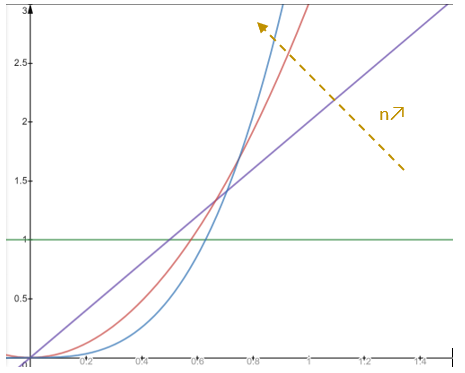
\includegraphics[scale = 0.6]{synthese_cm12_1.jpg}
        \end{figure}
    \end{minipage}
\end{example}

\begin{example}
    \begin{minipage}[c]{.55\linewidth}
        \begin{equation*}
            \begin{array}{c}
                \lim\limits_{n\to\infty}\int_0^1(1-x^{2n})nx^{n-1}dx=\lim\limits_{n\to\infty}\int_0^1(1-y^2)dy=\frac{2}{3}\\[0.4cm]
                \neq\\[0.4cm]
                \int_0^1\lim\limits_{n\to\infty}(1-x^{2n})nx^{n-1}dx=0
            \end{array}
        \end{equation*}
    \end{minipage}
    \begin{minipage}[c]{.4\linewidth}
        \begin{figure}[H]
            \centering
            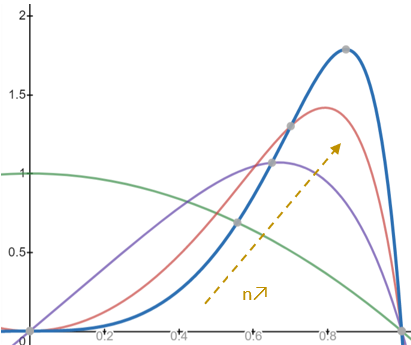
\includegraphics[scale = 0.6]{synthese_cm12_2.jpg}
        \end{figure}
    \end{minipage}
\end{example}

\begin{example}
    \begin{equation*}
        \lim_{n\to\infty}\int_{-\infty}^{+\infty}\frac{1}{1+(x-n)^2}dx=\lim_{n\to\infty}\int_0^1\frac{1}{1+y^2}dy=\pi \quad \neq\quad\int_{-\infty}^{+\infty}\lim_{n\to\infty}\frac{1}{1+(x-n)^2}dx=0
    \end{equation*}
    \begin{figure}[H]
        \centering
        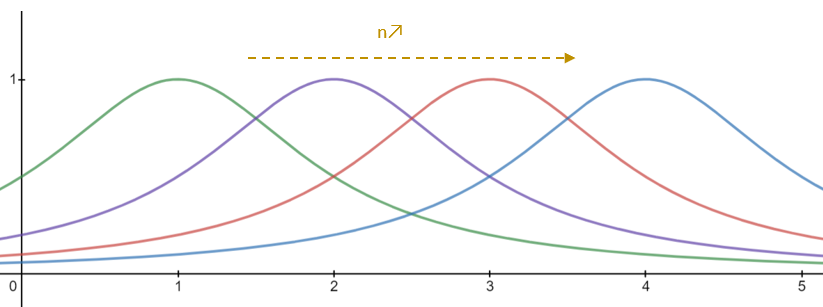
\includegraphics[scale = 0.6]{synthese_cm12_3.jpg}
    \end{figure}
\end{example}

\begin{example}
    \begin{equation*}
        \lim_{n\to\infty}\int_{-\infty}^{+\infty}\frac{n}{n^2+x^2}dx=\lim_{n\to\infty}\int_0^1\frac{1}{1+y^2}dy=\pi \quad\neq\quad\int_{-\infty}^{+\infty}\lim_{n\to\infty}\frac{n}{n^2+x^2}dx=0
    \end{equation*}
    \begin{figure}[H]
        \centering
        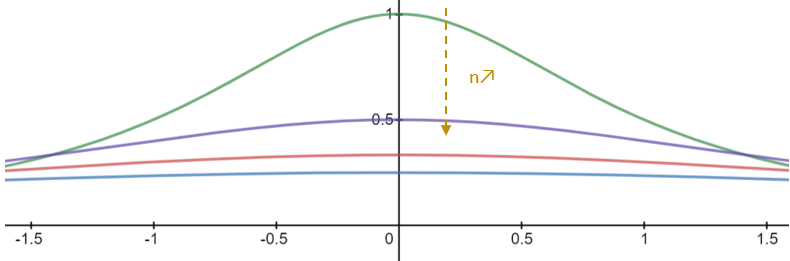
\includegraphics[scale = 0.6]{synthese_cm12_4.jpg}
    \end{figure}
\end{example}

\begin{theo}[Convergence monotone]
    Si $\forall n\in\mathbb{N}$, la fonction $f_n:X\to[0,\infty]$ est mesurable, $f_n\leq f_{n+1}$ partout sur $X$ et si $(f_n)_{n\in\mathbb{N}}$ converge ponctuellement vers $f$, alors $f$ est mesurable et on a
    \begin{equation*}
        \lim\limits_{n\to\infty}\int_A f_nd\mu = \int_Afd\mu.
    \end{equation*}
    \begin{figure}[H]
        \centering
        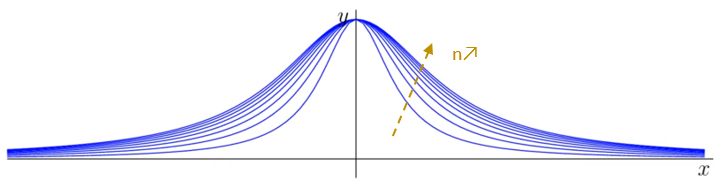
\includegraphics{synthese_conv_monotone.PNG}
    \end{figure}
\end{theo}
\begin{proof}
    On remarque tout d'abord que la suite $\big(\int_Af_nd\mu\big)_{n\in\mathbb{N}}$ est croissante et tend vers $\alpha\in[0,\infty]$. Puisque $f_n\leq f$, on sait que $\int_Af_nd\mu\leq\int_Afd\mu$ donc $\alpha\leq\int_Afd\mu$.
    
    On considère maintenant une fonction simple $s$ telle que $s\leq f$ et on pose $\theta\in]0,1[$. On définit ensuite l'ensemble $A_n=\{x\in A\big|f_n(x)\geq\theta s(x)\}$. Ces ensembles sont construits de manière à obtenir $A_n\subseteq A_{n+1}$ et $\bigcup_{n\in\mathbb{N}}A_n=A$. On observe donc que $\alpha\geq\int_Af_nd\mu\geq\int_{A_n}f_nd\mu\geq\int_{A_n}\theta sd\mu$. En faisant tendre $\theta$ vers $1$, on obtient que $\int_Asd\mu\leq\alpha$. Cette inégalité étant valable pour toute fonction simple, elle l'est aussi pour le supremum et on obtient finalement $\int_A fd\mu\leq\alpha$.
\end{proof}

\begin{theo}[Convergence dominée]
    Si $\forall n\in\mathbb{N}$, la fonction $f_n:X\to\mathbb{C}$ est telle que $(f_n)_{n\in\mathbb{N}}$ converge ponctuellement vers $f$ et si $\exists g:X\to[0,\infty[$ est intégrable sur $A$ et qu'on a la relation $|f_n|\leq g\ \forall n\in\mathbb{N}$, alors $f$ est intégrable et on a
    \begin{equation*}
        \lim\limits_{n\to\infty}\int_A f_nd\mu = \int_Afd\mu.
    \end{equation*}
    \begin{figure}[H]
        \centering
        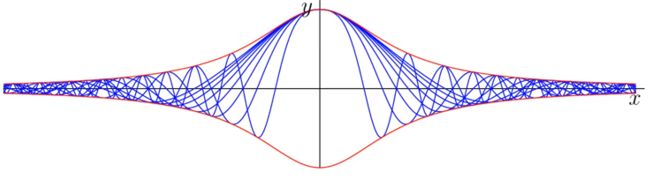
\includegraphics{synthese_conv_dominee.PNG}
    \end{figure}
    (comme $g$ est intégrable, l'aire sous sa courbe est finie et les fonctions $f_n$ doivent rester dans une partie du plan qui est finie)
\end{theo}
\begin{proof}
    Pour démontrer ce théorème, on va considérer des fonctions $f_n:X\to\mathbb{R}$.
    
    On définit pour chaque $n\in\mathbb{N}$ $\underbar{f}_n = \inf_{k\geq n}f_k$ et $\bar{f}_n = \sup_{k\geq n}f_k$. D'après le théorème de la convergence monotone, on a que $\lim\limits_{n\to\infty}\int_A\underbar{f}_n+g\ d\mu = \int_Af+g\ d\mu$ et $\lim\limits_{n\to\infty}\int_Ag-\bar{f}_n\ d\mu = \int_Ag-f\ d\mu$. Dès lors, $\lim\limits_{n\to\infty}\int_A\underbar{f}_nd\mu = \int_Afd\mu=\lim\limits_{n\to\infty}\bar{f}_nd\mu$. Grâce au théorème de l'étau, il est possible de conclure que $\lim\limits_{n\to\infty}\int_Af_nd\mu=\int_Afd\mu$.
\end{proof}

\begin{theo}[Réciproque de la convergence dominée]
    Si on a une suite de fonction $f_n:X\to[0,\infty[\ \forall n\in\mathbb{N}$ telle que $(f_n)_{n\in\mathbb{N}}$ converge ponctuellement vers $0$, et si $\lim\limits_{n\to\infty}\int_A f_nd\mu=0$, alors, $\exists g:X\to[0,\infty[$ intégrable sur $A$ et $\exists$ un suite strictement croissante $(n_k)_{k\in\mathbb{N}}$ dans $\mathbb{N}$ telle que $\forall k\in\mathbb{N}$, on ait $|f_{n_k}|\leq g$.
\end{theo}

\section{Différentiation et transformation de mesures}
\begin{theo}
    Si $f:X\to[0,\infty[$ est Borel-mesurable et si $\mu:\mathscr{B}(X)\to[0,\infty]$ est une mesure, alors $\nu:X\to[0,\infty]$ définie pour $A\in\mathscr{B}(X)$ par
    \begin{equation*}
        \nu(A)=\int_Afd\mu
    \end{equation*}
    est une mesure.
\end{theo}
\begin{proof}
    On remarque tout d'abord que $\nu(\emptyset)=\int_\emptyset fd\mu=0$.
    
    Ensuite, si on prend $A_n\in\mathscr{B}(X)$ disjoint, on a
    \begin{equation*}
        \nu\left(\bigcup_{n\in\mathbb{N}}A_n\right) = \int_{\bigcup_{n\in\mathbb{N}}A_n}fd\mu=\sum_{n\in\mathbb{N}}\int_{A_n}fd\mu = \sum_{n\in\mathbb{N}}\nu(A_n)
    \end{equation*}
\end{proof}

\begin{definition}
    Une mesure $\mu:Y\to[0,\infty]$ ($Y\in X$ est une $\sigma$-algèbre) est \textbf{$\sigma$-finie} si $\exists$ des ensembles $A_n\in Y$ tels qu'on peut écrire $X=\bigcup_{n\in\mathbb{N}}A_n$ avec $\mu(A_n)<\infty$.
\end{definition}

\begin{theo}[Radon-Nikodym]
    Si $\mu:\mathscr{B}(X)\to[0,\infty]$ est une mesure $\sigma$-finie et si $\nu:\mathscr{B}(X)\to[0,\infty]$ est absolument continue par rapport à $\mu$ ($\mu(A)=0\implies\nu(A)=0$), alors il existe une unique fonction $f:X\to[0,\infty]$ telle que $\forall A\in\mathscr{B}(X)$ on ait
    \begin{equation*}
        \nu(A)=\int_Afd\mu.
    \end{equation*}
    La fonction $f$ est appelée \textbf{dérivée de Radon-Nikodym} et est notée $\frac{d\nu}{d\mu}$. 
\end{theo}

\begin{remark}
    La continuité absolue est une hypothèse essentielle.
\end{remark}
\begin{example}
    Prenons $\mu=\lambda^1$, la mesure de Lebesgue sur $\mathbb{R}$ et $\nu$ la mesure de Dirac en $0$. Dès lors,
    \begin{equation*}
        \nu(\{0\}) = 1 \quad \neq \quad \int_{\{0\}}fd\mu=0
    \end{equation*}
    avec $f:X\to[0,\infty]$.
\end{example}

\begin{remark}
    La $\sigma$-finitude absolue est une hypothèse essentielle.
\end{remark}
\begin{example}
    Prenons $\mu$ la mesure de comptage ($\mu(A)=\#A=$ cardinal de $A=$ nombre d'éléments dans $A$) et $\nu=\lambda^1$ la mesure de Lebesgue. Dès lors, il devrait exister $a\in\mathbb{R}$ tel que $f(a)>0$ et on a alors $f(a)=\int_{\{a\}}fd\mu$ d'après la mesure $\mu$ or d'après la mesure $\nu=\int_{\{a\}}fd\mu$ on trouverais $0$...
\end{example}

\begin{definition}
    Si la fonction $f:X\to Y$ est Borel-mesurable et si $\mu:\mathscr{B}(X)\to[0,\infty]$ est une mesure, on définit la \textbf{mesure image} $f_*\mu:\mathscr{B}(Y)\to[0,\infty]$ par
    \begin{equation*}
        f_*\mu(A)=\mu\left(f^{-1}(A)\right)
    \end{equation*}
\end{definition}
\begin{proof}
    Tout d'abord, on remarque que cette fonction est bien définie car $f^{-1}(A)\in\mathscr{B}(X)$ si $A\in\mathscr{B}(Y)$.
    
    Ensuite, on vérifie que c'est bien une mesure :
    \begin{itemize}
        \item $f_*\mu(\emptyset)=\mu\big(f^{-1}(\emptyset)\big)=\mu(\emptyset)=0$ ;
        \item Considérons les ensembles $A_N\in\mathscr{B}(Y)$ disjoints,
        \begin{equation*}
            f_*\mu\left(\bigcup_{n\in\mathbb{N}}A_n\right)=\mu\left(f^{-1}\left(\bigcup_{n\in\mathbb{N}}A_n\right)\right)=\mu\left(\bigcup_{n\in\mathbb{N}}f^{-1}(A_n)\right) = \sum_{n\in\mathbb{N}}\mu\big(f^{-1}(A_n)\big) = \sum_{n\in\mathbb{N}}f_*\mu(A_n)
        \end{equation*}
    \end{itemize}
\end{proof}

\begin{example}
    Définissons $\mu$ par
    \begin{equation*}
        \mu(A) = \left\{\begin{array}{ll}
            1 & \text{si $a\in A$} \\
            0 & \text{sinon}
        \end{array}\right.
    \end{equation*}
    En utilisant la définition de la mesure image, on trouve
    \begin{equation*}
        f_*\mu(A) = \left\{\begin{array}{ll}
            1 & \text{si $a \in f^{-1}(A)$ ou encore si $f(a)\in A$} \\
            0 & \text{sinon}
        \end{array}\right.
    \end{equation*}
    Et la mesure de Dirac qu'on avait au départ reste une mesure de Dirac.
\end{example}

\begin{theo}
    Si $f:X\to Y$ et $g:Y\to\mathbb{C}$ sont Borel-mesurable alors $g$ est intégrable sur $A\subseteq Y$ par rapport à $f_*\mu$ si et seulement si $g\circ f$ est intégrable sur $f^{-1}(A)\subseteq X$ par rapport à $\mu$ et
    \begin{equation*}
        \int_Ag\ d(f_*\mu) = \int_{f^{-1}(A)}g\circ f \ d\mu
    \end{equation*}
\end{theo}
\begin{proof}
    Si $s$ est une fonction simple, $(s\circ f)^{-1}(\{\alpha_i\}) = f^{-1}\big(s^{-1}(\{\alpha_i\})\big)$ et donc $\mu\big((s\circ f)^{-1}(\{\alpha_i\})\big)=f_*\mu\big(s^{-1}(\{\alpha_i\})\big)$.
\end{proof}

\begin{theo}
    Si $f(x)=Mx+a$ avec $M$ une matrice inversible, on a
    \begin{equation*}
        f_*\lambda^{n} = \frac{1}{|\det M|}\lambda^n
    \end{equation*}
\end{theo}
\begin{proof}
    Si $A,B\in\mathscr{B}(\mathbb{R}^n)$, on obtient en échangeant les ordres d'intégration et en effectuant des changements de variables par translation :
    \begin{align*}
        \lambda^n(A)(f_*\lambda^n)(B) &= \iint_{\mathbb{R}^n\times\mathbb{R}^n} \chi_A(x)\chi_{f^{-1}(B)}(y)\ dydx 
        = \iint_{\mathbb{R}^n\times\mathbb{R}^n} \chi_A(x)\chi_{B}(My+a)\ dydx \\
        &= \iint_{\mathbb{R}^n\times\mathbb{R}^n} \chi_A(x)\chi_{B}\big(M(y-M^{-1}x)+a\big)\ dydx \\
        &= \iint_{\mathbb{R}^n\times\mathbb{R}^n} \chi_A(x)\chi_{B}(My-x+a)\ dydx
        = \iint_{\mathbb{R}^n\times\mathbb{R}^n} \chi_A(My+a-z)\chi_{B}(z) dydz\\
        & = \iint_{\mathbb{R}^n\times\mathbb{R}^n} \chi_A\big(M(y-M^{-1}z)+a\big)\chi_{B}(z) dydz\\
        &= \iint_{\mathbb{R}^n\times\mathbb{R}^n} \chi_A(My+a)\chi_{B}(z) dydz
        = \iint_{\mathbb{R}^n\times\mathbb{R}^n} \chi_{f^{-1}(A)}(y)\chi_{B}(z) dydz\\
        & = (f_*\lambda^n)(A)\lambda^n(B)
    \end{align*}
    On en déduit donc que
    \begin{equation*}
        f_*\lambda^{n}(A) = \frac{f_*\lambda^{n}(B)}{\lambda^n(B)}\lambda^n(A).
    \end{equation*}
    Ensuite, en considérant que $M$ est une matrice diagonale, on a que l'ensemble $B$ est un pavé et on retrouve la formule énoncé plus haut. Si on considère une matrice $M$ orthogonale, on prend pour l'ensemble $B$ une boule. Dans le cas général, on remarque qu'une matrice quelconque s'écrit comme le produit de matrices orthogonales et diagonales et on retrouvera donc toujours la formule désirée.
\end{proof}

\begin{theo}
    De manière plus générale, si $f:U\to V$ est un difféomorphisme de classe $C^1$ : $f$ est continuement différentiable, inversible et $f^{-1}$ est continuement différentiable, alors on a
    \begin{equation*}
        f_*\lambda^n = \frac{1}{|\det df|\circ f^{-1}}\lambda^n
    \end{equation*}
\end{theo}